\chapter{GPU and Clock Unit design}

\section{GPU}
The GPU bears its name rather badly because it is not really programmable. But this is the only name 
that was found for it and therefore kept. This unit provides a 
graphic memory and the tools to draw patterns of 8x8 pixels, called masks. The writing in this 
memory is done from the beta machine (the CPU) through the store instruction (ST). The specific way 
of addressing the memory and the structure of the commands are described later. As far as the colors 
are concerned, it has been decided to work with 12 bit RGB colors, that is to say 4 bits per primary 
color.

In addition to this, the GPU also provides the HDMI controller. This controller simply reads the 
graphic memory in loop and draws its content on the screen. The controller handles a 
16:9 screen using a resolution of 848x480 pixels and a refresh rate of 60Hz. The protocol used is 
the VESA 848x480, it is described later. 

Before moving on to the description of the different modules making up the GPU, a description of 
how the screen and the masks are interpreted by the GPU is done. The VESA protocol is also detailed.

\subsection{Screen and tile representation}

As said before, the masks are 8x8 pixels and the goal is to be able to apply them anywhere on the 
screen. 
The screen is therefore naturally divided into a set of 8x8 pixels squares which are called tiles. 
In memory, the idea is that there are 3 sub-memories whose words contain a color of the three 
primary colors (red, green or blue) of a whole tile. A tile corresponding to 64 pixels and a 
primary color being coded on 4 bits, it gives words of 256 bits. Then, by dividing the dimensions 
of the screen (848x480 pixels) by 8, one finds that 106x60 tiles, so 6360, are enough to represent 
the screen. In order not to use too much memory, it is decided to use 72x54 tiles. This corresponds 
to the largest integer size allowing a 4:3\footnote{This ratio corresponds to the ration between the
width and the height, in terms of tiles, of the useful screen. This has nothing to do with the 
resolution ratio of the screen that is 16:9.} ratio with a maximum use of 4096 tiles.  It is decided 
to limit to 4096 tiles because to use 6360 tiles it would be necessary to have a memory with 8192 
words, which would use too much memory unnecessarily. The useful screen is centered in the physical 
screen. Figure \ref{fig:gpu/screen_size} summarizes all this.

\begin{figure}[H]
    \centering
    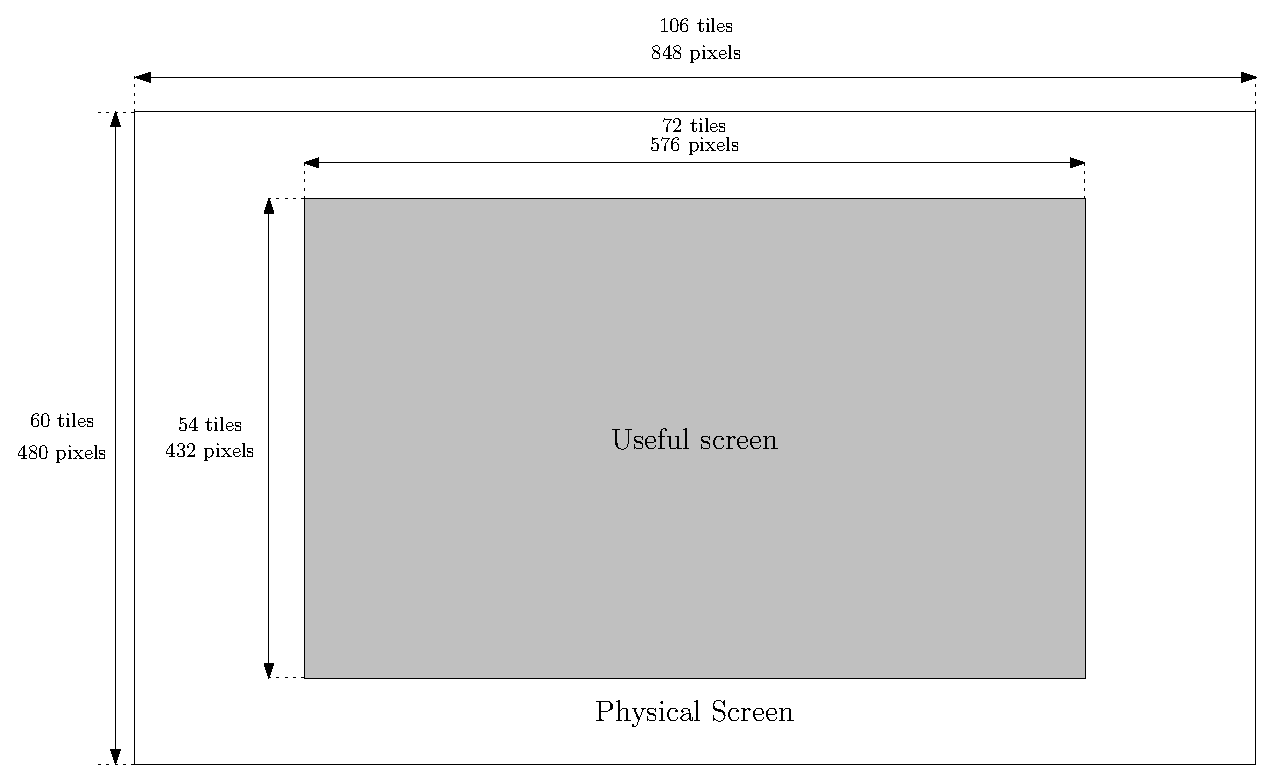
\includegraphics[width=\linewidth]{Chapter4-GPU_CLKU/res/screen_size}
    \caption{Useful screen area in the physical screen}
    \label{fig:gpu/screen_size}
\end{figure}

The problem with putting all tiles in a single memory like this is that only one tile is accessible 
at a time. This means that a mask can only be applied to one tile. This is a pity because it 
prevents the mask from being drawn anywhere on the screen. Indeed, the mask cannot for example be 
drawn between two tiles as shown in Figure \ref{fig:gpu/mask_2tiles}.

\begin{figure}[H]
    \centering
    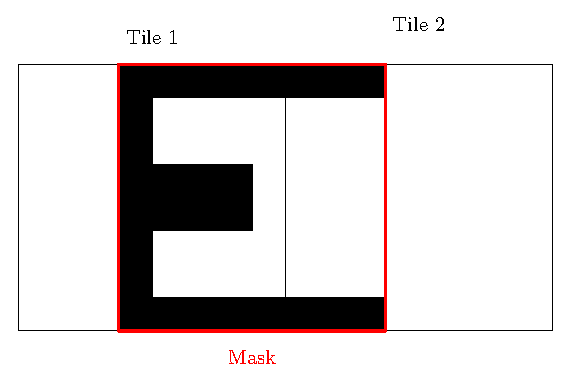
\includegraphics[scale=1.0]{Chapter4-GPU_CLKU/res/mask_2tiles}
    \caption{Mask overlapping two tiles}
    \label{fig:gpu/mask_2tiles}
\end{figure}

When such a placement of the mask takes place, what actually happens is a tile is chosen first. And 
then an offset in pixels is added to the mask. In the example in Figure \ref{fig:gpu/mask_2tiles}, 
the mask has a positive 
offset of N pixels with respect to Tile 1. The idea is then to allow a mask to have an abscissa and
an ordinate offset ranging from 0 to 7. It is not useful to go further than 7 
as this corresponds to placing the mask at the next tile. To be able to apply the mask, it is 
therefore necessary to be able to load four tiles. The first one being the one chosen to draw the 
mask in (x, y), the others being those in (x + 1, y), (x, y + 1) and (x + 1, y + 1). A naive 
solution to load these four tiles would be to have a memory for each tile. However, this has two 
problems. The first one is that this is impossible for the Cyclone V. Indeed, it was seen earlier that 
the Cyclone V has just over 500 M10K memory blocks. However, to represent all the tiles, one would 
need 3888 memories because the definition of a memory in the code must use at least one whole M10K, 
which is simply impossible. Secondly, this would generate way to many connections in the circuits
and a complex multiplexing stage in the memory circuits. This is not tractable for the Cylone V 
neither.

Another way is to try to divide the set of tiles into four groups. These four groups should be 
distributed on the screen in such a way that the placement of a mask loads 4 tiles of different 
groups each time. If one thinks about it, it is possible to convince itself that a simple paving 
of 4 colors allows this (a color represents a group). Figure \ref{fig:gpu/screen_tiling} shows such 
a tiling. 

\begin{figure}[H]
    \centering
    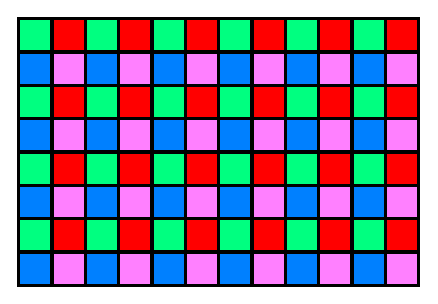
\includegraphics[scale=1.0]{Chapter4-GPU_CLKU/res/screen_tiling}
    \caption{Screen tiling}
    \label{fig:gpu/screen_tiling}
\end{figure}

And the different cases possible by choosing four tiles in the way explained earlier, i.e. one 
tile, the one to the right of it, the one below it and the one at the bottom right are shown in
Figure \ref{fig:gpu/screen_tiling_cases}. It can be seen that in each case, a group is present only 
once, which validates the possibility of representing all tiles using four distinct memories.

\begin{figure}[H]
    \centering
    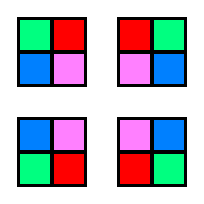
\includegraphics[scale=1.0]{Chapter4-GPU_CLKU/res/screen_tiling_cases}
    \caption{Screen tiling selection cases}
    \label{fig:gpu/screen_tiling_cases}
\end{figure}

\subsection{Mask representation}

A mask has the same dimensions as a tile but does not have the same content. Indeed, a mask can 
contain four different values. The first value is \textit{keep}, corresponding to a 0 in the mask. This 
value means that no modification is made to the pixel targeted by this position in the 
mask. Then there is \textit{set primary}, corresponding to 1, which sets the pixel at this 
location to the primary color, this is better explained later. When the value is 2, 
for \textit{set secondary}, it is then the secondary color that is applied. And 
finally, for the value 3 corresponding to a \textit{reset}, the pixel becomes black. Each of these 
values can therefore be represented on 2 bits. Table \ref{tab:mask_op} summarizes the possible 
operations of a mask.
% PF In general here, I do not see well the constraints imposed by the material vs the design choices.
% PF I am a bit confused: I do not understand the relation to the 4 bits per color in the graphic memory and the primary/secondary color in masks
% PF This is made clear later...


\begin{table}[H]
    \centering
    \begin{tabular}{|l|c|}
    \hline
    \rowcolor[HTML]{DAE8FC} 
    \multicolumn{1}{|c|}{\cellcolor[HTML]{DAE8FC}\textbf{Mask Operation}} & \textbf{Mask Value} \\ \hline
    Keep                                                                  & 0b00                \\ \hline
    Set primary                                                           & 0b01                \\ \hline
    Set secondary                                                         & 0b10                \\ \hline
    Reset                                                                 & 0b11                \\ \hline
    \end{tabular}
    \caption{Mask operations}
    \label{tab:mask_op}
\end{table}

In terms of representation, a mask is a simple vector of 8x8x2 (128) bits. Its LSB corresponds to 
the upper left corner of the mask and its MSB corresponds to the lower right corner of the mask. 
This correspondence is shown in Figure \ref{fig:gpu/mask_vector}.

\begin{figure}[H]
    \centering
    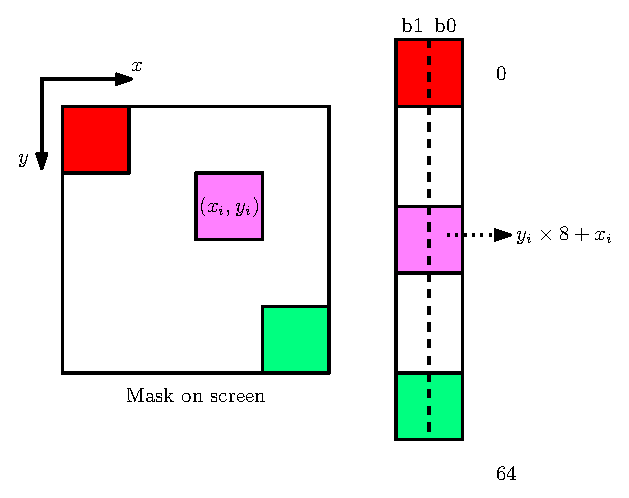
\includegraphics[scale=1.0]{Chapter4-GPU_CLKU/res/mask_vector}
    \caption{Mask vector representation}
    \label{fig:gpu/mask_vector}
\end{figure}

\subsection{Using the GPU}

As introduced, to use the GPU, it is necessary to use the store instruction from the CPU. But the 
address and data must be correctly formatted. For the address, it must start with 0b10 as seen in 
the chapter on the CPU (so that the addressed unit is the GPU). Then, it was decided to make the 
address natural, that is to say that it is 
readable without any conversion. The address therefore contains the exact pixel position where 
a mask should be applied. A pixel being located by four variables: block\_x, block\_y (corresponding 
to the tile), off\_x and off\_y (corresponding to the offset from the tile), these four variables 
are directly present in the address. The format of the address is detailed in 
Figure \ref{fig:gpu/store_address}.

\begin{figure}[H]
    \centering
    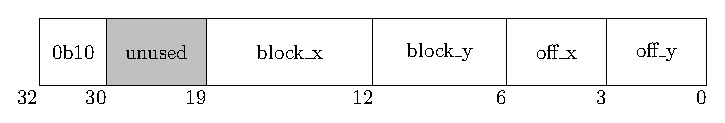
\includegraphics[scale=1.0]{Chapter4-GPU_CLKU/res/store_address}
    \caption{Store instruction address}
    \label{fig:gpu/store_address}
\end{figure}

Concerning the data writen by the store instruction, it must contain the mask identifier and the 
values of the two colors. As a color is 
represented on 12 bits and a word on the CPU is represented on 32 bits, 8 bits remain for the mask.  
The GPU can therefore support 256 masks. The data format is detailed in 
Figure \ref{fig:gpu/store_data}.

\begin{figure}[H]
    \centering
    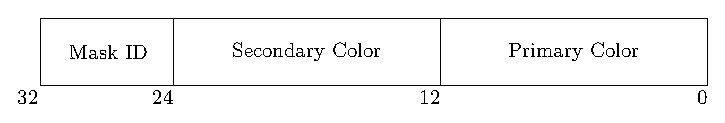
\includegraphics[scale=1.0]{Chapter4-GPU_CLKU/res/store_data}
    \caption{Store instruction data}
    \label{fig:gpu/store_data}
\end{figure}

\subsection{VESA protocol}

The VESA protocol works exactly like the VGA protocol. That is, four signals are present. On the 
one hand there is the 24 bit color signal (8 bits for each primary color, only 4 are truly used
here, the least significant bits are replaced by zeros), the vertical and 
horizontal synchronization signals and the display enable signal. The synchronization signals 
inform the screen of the end of a line for horizontal synchronization and the end of a frame (all 
the lines on a screen) for vertical synchronization. Between two horizontal synchronization 
signals, several things happen. First, there is a pause just after the signal. This time is called 
horizontal back porch. Then, after this pause the colors are sent, the value must be maintained for 
a certain time to fix a pixel. All the pixels of the line are assigned one after the other, in a 
burst. Of course there are specific timing criteria that must be met for this to work, this is 
discussed next. After sending all the colors, a new pause takes place, called horizontal front 
porch. And finally, after this pause, a new horizontal synchronization signal is sent. For the 
frames, it is similar. Before the frame, there is a pause (vertical front porch) followed by the 
vertical synchronization followed by the vertical back porch. Note that the horizontal and vertical 
synchronizations are independent, so both must be evaluated at each moment. When no pause or 
synchronization occurs, either horizontal or vertical, the display is said to be enable. The 
display enable signal is then high and the colors are actually used for the pixels. Outside this 
condition, the color signal can be set to any value and is not listened to. 

The operation of the protocol is shown in Figure \ref{fig:gpu/screen_vesa}. The legend and length
of the signals are available in Table \ref{tab:gpu/vesa}. In this figure, 
the protocol is described in relation to the pixels, and therefore the position on the screen. As 
the screen only includes the pixels of the region where display enable is high, the frame shown is 
a virtual screen, not the physical one, which is smaller. The description is made in relation to the 
pixels because 
it is easier to understand but also to implement. Indeed, as shown later in this report, pixel 
counters are sufficient to implement this protocol. Then, it is enough to fix the right clock 
frequency so that the timings of each pixel are respected. For VESA 848x480, a  33.750MHz clock
is used. Figure \ref{fig:gpu/vesa_signals} shows the value of the signals according to the position
on the screen.

\begin{figure}[H]
    \centering
    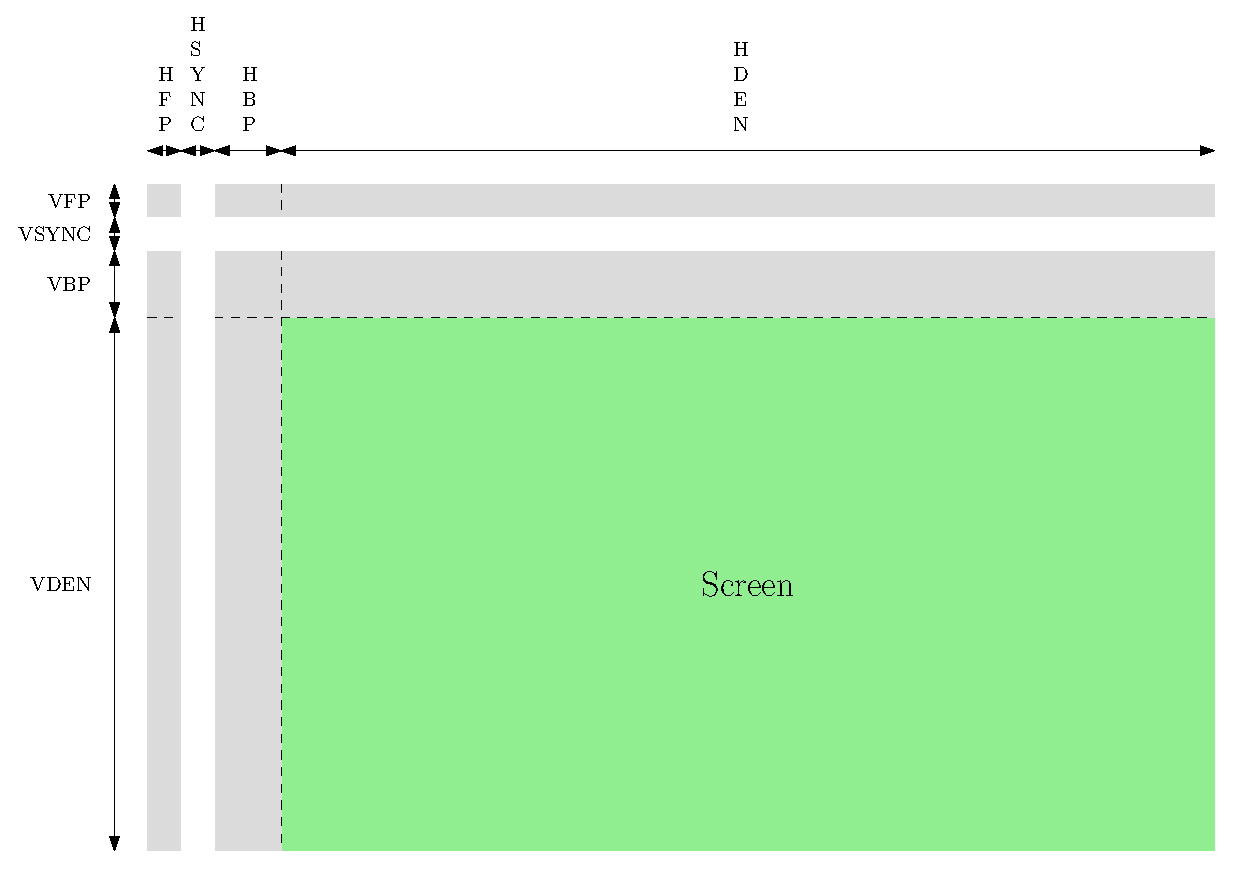
\includegraphics[width=\linewidth]{Chapter4-GPU_CLKU/res/screen_vesa}
    \caption{VESA virtual screen schematic}
    \label{fig:gpu/screen_vesa}
\end{figure}

\begin{table}[H]
    \centering
    \begin{tabular}{|c|c|c|}
    \hline
    \rowcolor[HTML]{DAE8FC} 
    \textbf{Signal} & \textbf{Complete name}    & \multicolumn{1}{l|}{\cellcolor[HTML]{DAE8FC}\textbf{Length (pixels)}} \\ \hline
    HFP             & Horizontal Front Porch    & 16                                                                    \\ \hline
    HSYNC           & Horizontal Sync           & 112                                                                   \\ \hline
    HBP             & Horizontal Back Porch     & 112                                                                   \\ \hline
    HDEN            & Horizontal Display Enable & 848                                                                   \\ \hline
    VFP             & Vertical Front Porch      & 6                                                                     \\ \hline
    VSYNC           & Vertical Sync             & 8                                                                     \\ \hline
    VBP             & Vertical Back Porch       & 23                                                                    \\ \hline
    VDEN            & Vertical Display Enable   & 480                                                                   \\ \hline
    \end{tabular}
    \caption{VESA 848x480 counts}
    \label{tab:gpu/vesa}
\end{table}

\begin{figure}[H]
    \centering
    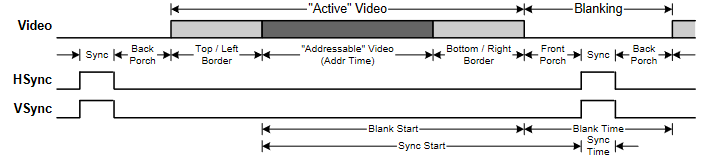
\includegraphics[width=\linewidth]{Chapter4-GPU_CLKU/res/vesa_signals.PNG}
    \caption{VESA signals - video signal represents both display enable signals}
    \label{fig:gpu/vesa_signals}
\end{figure}

\section{GPU components}

\subsection{Graphic memory}

The graphic memory has two functions. The first one is of course to store the state of all the 
pixels of the screen. This is done as discussed above by splitting the memory into four parts. One 
for each group of the Figure \ref{fig:gpu/screen_tiling} tiling. Each of these sub-memories is then 
divided into three memories, one for 
each primary color. This was done this way because it is more optimal to have three memories whose 
word size is a power of two. By dividing by three, each word has 4 bits while it would have had 
12 bits in the case of full colors, which is not a power of 2. A fifth port with a different clock 
from the first 4 ports is also exposed by the graphic memory. This one allows the reading of the 
memory tile by tile for the HDMI controller part of the GPU. This operation is completely independent
of the CPU accesses of this memory, that is why another port is used. The tile loaded from this port
is referred to as Tile b.

The second function is to correctly direct the values in memory to the outputs when reading, and 
the values in input to the memories when writing. Indeed, depending on the editing position (address), the 
current tile belongs to one of the memories. And the memories of the other three tiles to be 
selected also depends on this position. See Figure \ref{fig:gpu/screen_tiling_cases} for the different 
possible configurations. 

From now on, the current tile (at the target position) will be tile 0. The one to the right of it
will be tile 1, the one below it will be tile 2 and the one below it on the right will be tile 3. 
Figure \ref{fig:gpu/tile_ids} summarizes this. Note that the colors are set by tiles. A memory word 
is therefore $4 \times 64$ = 256 bits.

\begin{figure}[H]
    \centering
    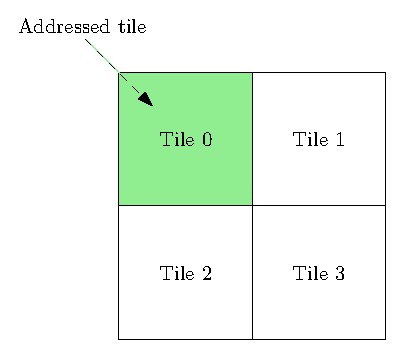
\includegraphics[scale=1.0]{Chapter4-GPU_CLKU/res/tile_ids}
    \caption{Tile identifiers}
    \label{fig:gpu/tile_ids}
\end{figure}

\subsubsection*{Memory unit}

The memory units are the modules representing the groups of tiles, so there are 4 of them in the 
graphic memory. Each memory unit is composed of three Altsyncram configured in true-dualport RAM 
representing the three primary colors. True dualport means that they come with two completely 
independent ports whose clocks are different. The module simply interfaces these three Altsyncrams. 
The internal circuit is given in Figure \ref{fig:gpu/memory_unit_in} and its interface in Figure 
\ref{fig:gpu/memory_unit}. As can be seen, the wren\_b and data\_b signals 
of each memory are grounded since the second port is read-only, that is the one corresponding to
Tile b. The HDMI controller doesn't need to write in memory. For the rest, the signals are 
simply retransmitted. The addresses in the three internal memories are the same since it is the
same tile that is targeted each time. The words are all 256 bits long as each word contains 64 
pixels and one of their color components on 4 bits. 

Now that the memory units are described, it is possible to establish the complete memory circuit.
The complete circuit is shown in Figure \ref{fig:gpu/memory_in}. It consists of a parallel 
connection of four memory units. 

Each color input of each memory unit is multiplexed between the four color inputs of the same color. 
The four inputs of these multiplexers are in fact the colors of each of the 
tiles used (tile 0, tile 1, tile 2 and tile 3). Then, each of the outputs of the memory are 
multiplexed from the values in memory in the different memory units. All these multiplexers ensure 
that the tiles are correctly routed, as explained above. These multiplexers are controlled by five 
signals: sw0, sw1, sw2, sw3 and swb which are respectively linked to tile 0, tile 1, tile 2, tile 3 
and tile b. The determination of the values of these switches as well as those of the addresses of 
the memory units are not displayed in the circuit for simplicity. But their
value are simply based on the selected tile location, Tile 0. Depending on its location, it belongs 
to one of the four tile groups. The groups of the neighbor tiles are also computed based on the 
locations of these tiles and their respective switches are set according to the group of the tile. 

\begin{figure}[H]
    \centering
    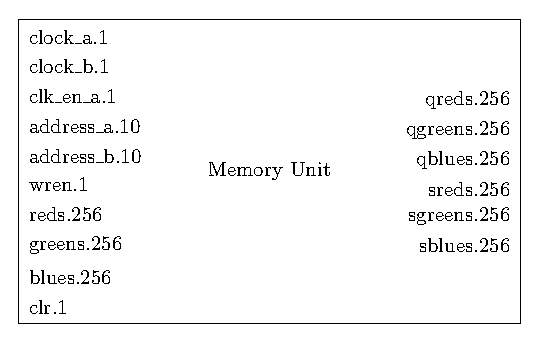
\includegraphics[scale=1.0]{Chapter4-GPU_CLKU/res/memory_unit}
    \caption{Memory Unit}
    \label{fig:gpu/memory_unit}
\end{figure}

\begin{figure}[H]
    \centering
    
\includegraphics[scale=1.0]{Chapter4-GPU_CLKU/res/memory_unit_in}
    \caption{Memory Unit internal circuit}
    \label{fig:gpu/memory_unit_in}
\end{figure}

\begin{figure}[H]
    \centering
    
\includegraphics[scale=0.55]{Chapter4-GPU_CLKU/res/memory_in_part1}
    \caption{Memory internal circuit}
    \label{fig:gpu/memory_in}
\end{figure}

The interface of the memory can be found in Figure \ref{fig:gpu/memory}. 
The red, green and blue signals of each tile 
are put together in a bus to simplify the representation of the module.

\begin{figure}[H]
    \centering
    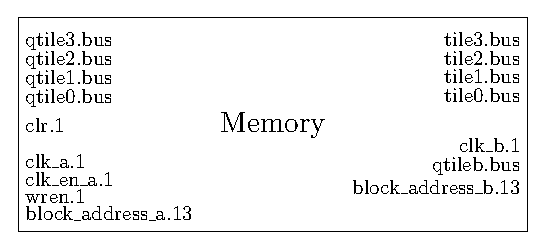
\includegraphics[scale=1.0]{Chapter4-GPU_CLKU/res/memory}
    \caption{Memory}
    \label{fig:gpu/memory}
\end{figure}

\subsection{Mask memory}

The mask memory is identical to the CPU instruction memory except that the Altsyncram used contains 
only 256 words of 128 bits. This allows to store 256 masks. The circuit is given in Figure
\ref{fig:gpu/mask_memory_in} and \ref{fig:gpu/mask_memory} provides its interface. Note that if the 
address is equal to 255, then the mask sent to the data\_read output is a constant mask 
(named clear mask) which clears all pixels.

\begin{figure}[H]
    \centering
    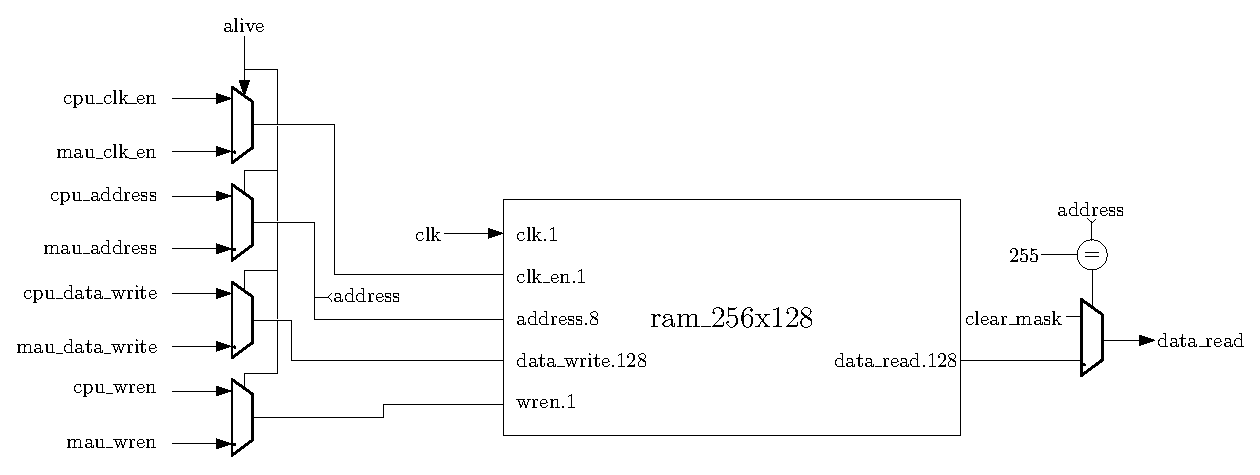
\includegraphics[width=\linewidth]{Chapter4-GPU_CLKU/res/mask_memory_in}
    \caption{Mask memory internal circuit}
    \label{fig:gpu/mask_memory_in}
\end{figure}

\begin{figure}[H]
    \centering
    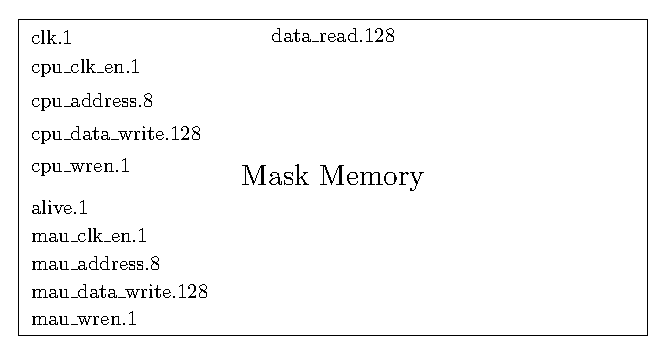
\includegraphics[scale=0.8]{Chapter4-GPU_CLKU/res/mask_memory}
    \caption{Mask memory}
    \label{fig:gpu/mask_memory}
\end{figure}

\subsection{Shifter}

The objective of this module is to replicate the mask four times and to shift it in each of these 
copies so that it corresponds to the mask offset given by the user. After that, each of the copies 
can be associated with one of the four tiles loaded out of memory. This association is done in 
another module.

\subsubsection*{Shifter Unit}

This module is responsible for shifting. To do this it simply takes the signed 
offsets given in input and shifts the bits of the mask. The offsets being given in pixels and the
masks having two bits per pixel, it is necessary to multiply by two each offset. To achieve an 
horizontal offset, each line of the mask is shifted 2 $\times$ offset\_x while for a vertical offset, the whole mask is shifted of 16 $\times$ offset\_y given that there are 8 pixels 
by line. The circuit and the interface of the shifter unit are respectively given in Figures
\ref{fig:gpu/shifter_unit_in} and \ref{fig:gpu/shifter_unit}.

\begin{figure}[H]
    \centering
    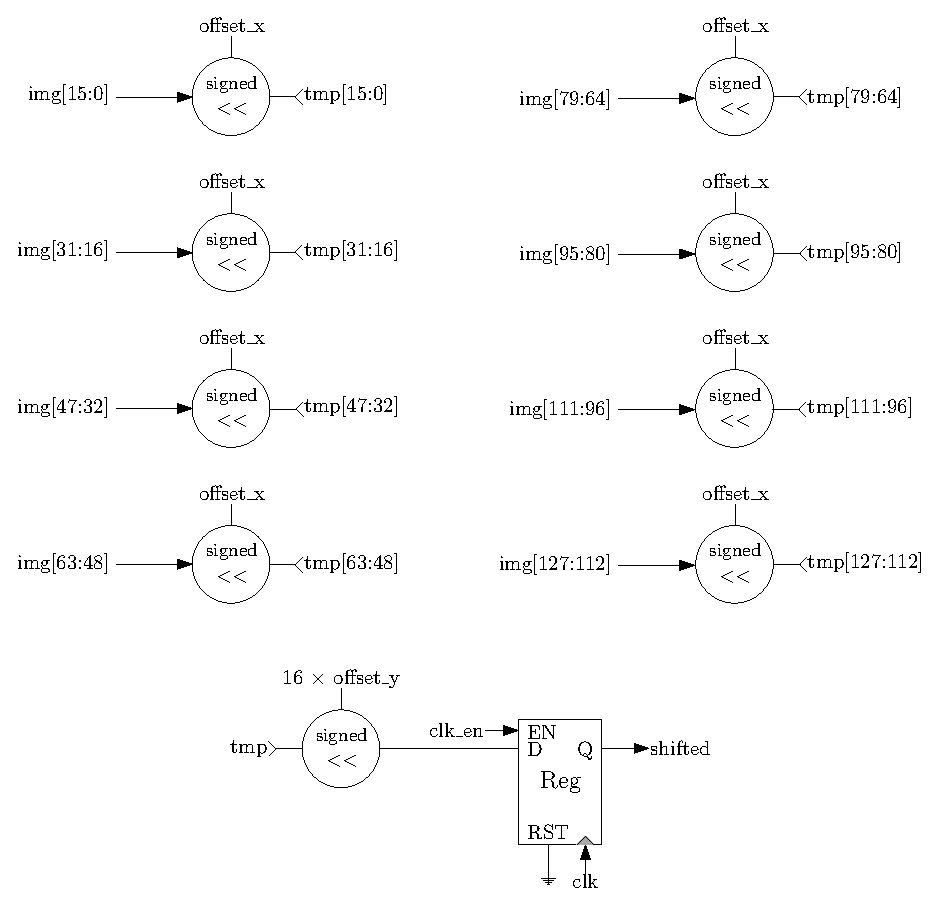
\includegraphics[width=\linewidth]{Chapter4-GPU_CLKU/res/shifter_unit_in}
    \caption{Shifter unit internal circuit}
    \label{fig:gpu/shifter_unit_in}
\end{figure}

\begin{figure}[H]
    \centering
    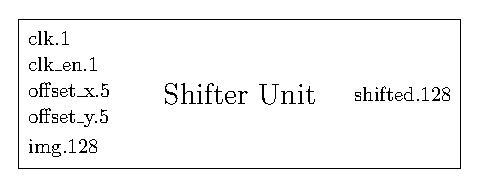
\includegraphics[scale=0.8]{Chapter4-GPU_CLKU/res/shifter_unit}
    \caption{Shifter unit}
    \label{fig:gpu/shifter_unit}
\end{figure}

The complete shifter is just a simple parallelization of four shifters but one has to choose the right 
offsets for each shifter unit. In Figure \ref{fig:gpu/shifter_offsets} are shown
the different offsets needed to obtain the desired masks. Each offset is taken with respect to the 
upper left corner of the mask to which it is associated. off\_0 is of course equal to 
(off\_x, off\_y) since the offset is always given from the selected tile and the selected tile is 
identified by id 0. For the others, the offsets are off\_1 = (off\_x - 8, off\_y), off\_2 = 
(off\_x, off\_y - 8) and off\_3 = (off\_x - 8, off\_y - 8).

\begin{figure}[H]
    \centering
    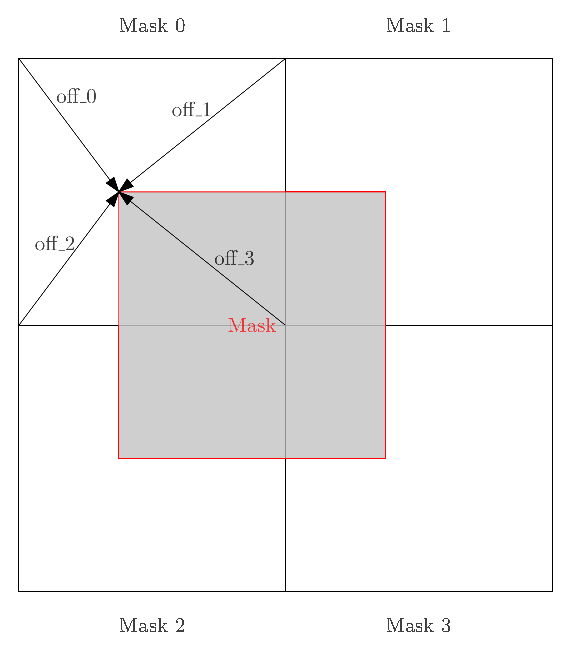
\includegraphics[scale=1.0]{Chapter4-GPU_CLKU/res/shifter_offsets}
    \caption{Masks offsets}
    \label{fig:gpu/shifter_offsets}
\end{figure}

The complete shifter circuit can then be established and is given in Figure \ref{fig:gpu/shifter_in}. 
Figure \ref{fig:gpu/shifter} contains the shifter interface.

\begin{figure}[H]
    \centering
    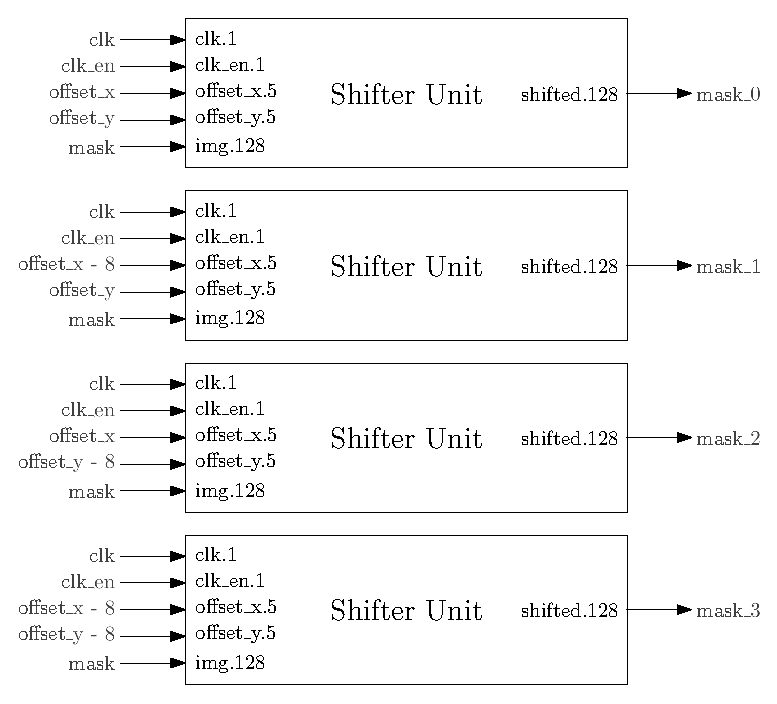
\includegraphics[scale=1.0]{Chapter4-GPU_CLKU/res/shifter_in}
    \caption{Shifter internal circuit}
    \label{fig:gpu/shifter_in}
\end{figure}

\begin{figure}[H]
    \centering
    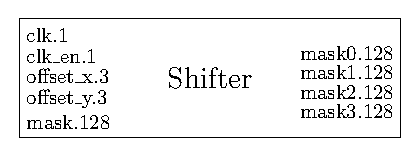
\includegraphics[scale=1.0]{Chapter4-GPU_CLKU/res/shifter}
    \caption{Shifter}
    \label{fig:gpu/shifter}
\end{figure}


\subsection{Mask Logic Unit (MLU)}

The MLU is simply used to modify the current value of a pixel in a tile according to the operation 
described for this pixel in the corresponding mask. This module is a kind of giant multiplexer. In 
fact, it contains a multiplexer for each primary color of each pixel and will select an input 
(the current value of the pixel, the primary color, the secondary color or the black color) 
according to the value of the mask at that position. Its operation is very simple to understand 
and its circuit impossible to draw on a page of this report, so the circuit is not detailed here. The interface is however given in Figure \ref{fig:gpu/mlu}.
Note that this circuit is completely combinatorial. Concerning the tile buses, they are simply
made up of the three color signals of the corresponding tile.

\begin{figure}[H]
    \centering
    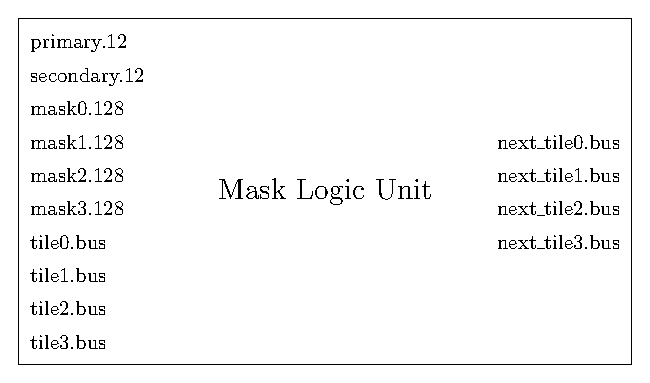
\includegraphics[scale=1.0]{Chapter4-GPU_CLKU/res/mlu}
    \caption{Mask Logic Unit}
    \label{fig:gpu/mlu}
\end{figure}

\subsection{Graphic Counter (GC)}

The graphics counter is the first element fully included in the HDMI controller part of the GPU. 
It simply counts and provides several counts. First, it provides the current position of the 
pixel taken into account, so cnt\_h and cnt\_v representing the horizontal and vertical position 
of the pixel. These go through all the virtual screen of the VESA, that is to say from 0 to 1087 
for cnt\_h and from 0 to 516 for cnt\_v. These counts are then used to correctly generate the 
synchronization signals of the VESA in another module. 

Then, it provides four other counters blk\_x, blk\_y, off\_x, off\_y which again give the position 
of a pixel but using this time the GPU coordinate system. It should be noted that these counters 
only count from the start of the useful screen. In other words, blk\_x and blk\_y are both at 0 
when cnt\_h and cnt\_v correspond to the location of the first pixel of the first tile in 
memory, the one at the top left corner of the useful screen. And their values continue to increase 
until the end of the VESA virtual screen.

Notice also that the useful screen does not correspond to the entire active area of the 
VESA. As mentioned earlier, not all the space is used because of memory constraints. The useful 
screen is centered in this active region. When the counter is in the useful region of the screen, 
the in\_mem signal is high to warn that the position given by the counter corresponds to a tile 
present in memory. The range of the counters and a schematic of the positioning of the useful 
region are given in Figure \ref{fig:gpu/gc_screen}.

\begin{figure}[H]
    \centering
    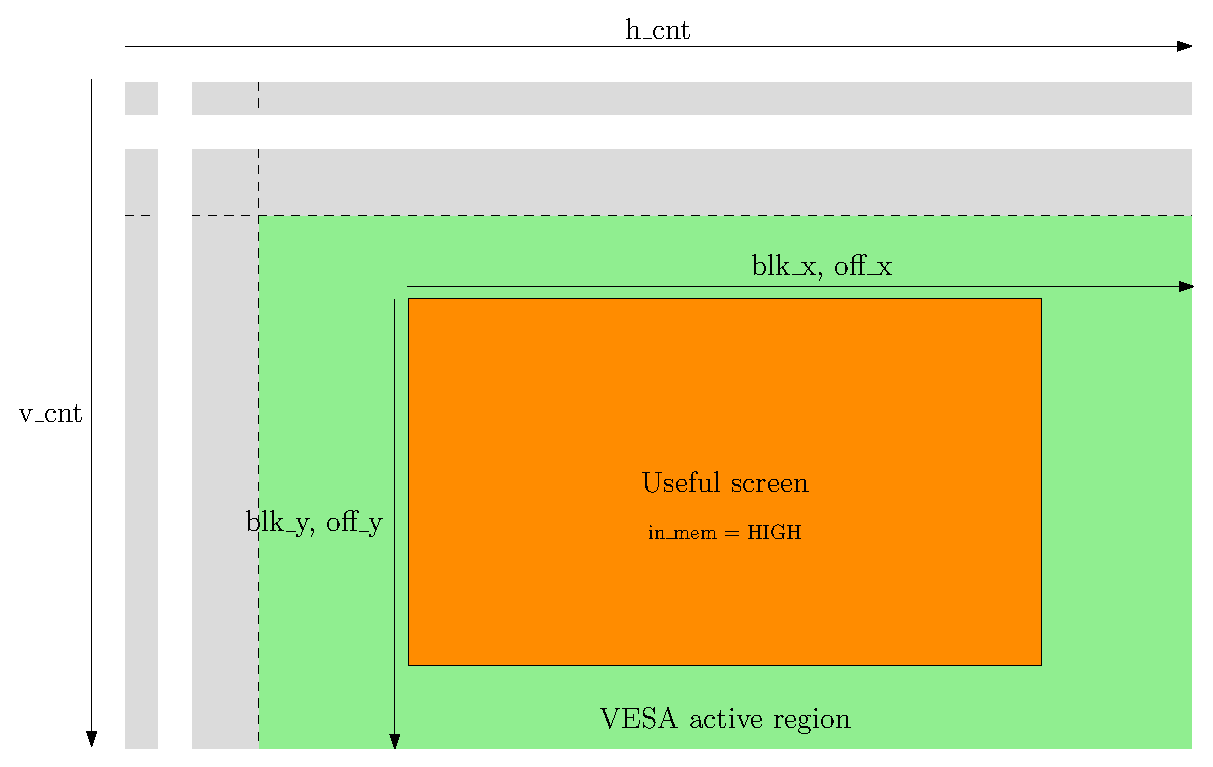
\includegraphics[width=\linewidth]{Chapter4-GPU_CLKU/res/gc_screen}
    \caption{Counters range and useful screen}
    \label{fig:gpu/gc_screen}
\end{figure}

All these counters are implemented with the help of registers by choosing correctly the clk\_enable 
signals and the reset signals. The inner circuit without the in\_memory which is only a condition 
on the values of h\_cnt and v\_cnt is given in Figure \ref{fig:gpu/gc_in}. The interface is also shown in Figure \ref{fig:gpu/gc}.

\begin{figure}[H]
    \centering
    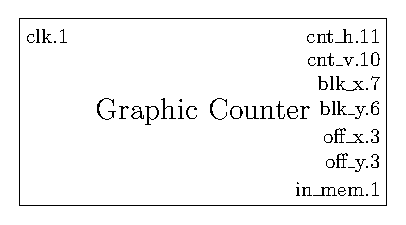
\includegraphics[scale=0.8]{Chapter4-GPU_CLKU/res/gc}
    \caption{Graphic counter}
    \label{fig:gpu/gc}
\end{figure}

\begin{figure}[H]
    \centering
    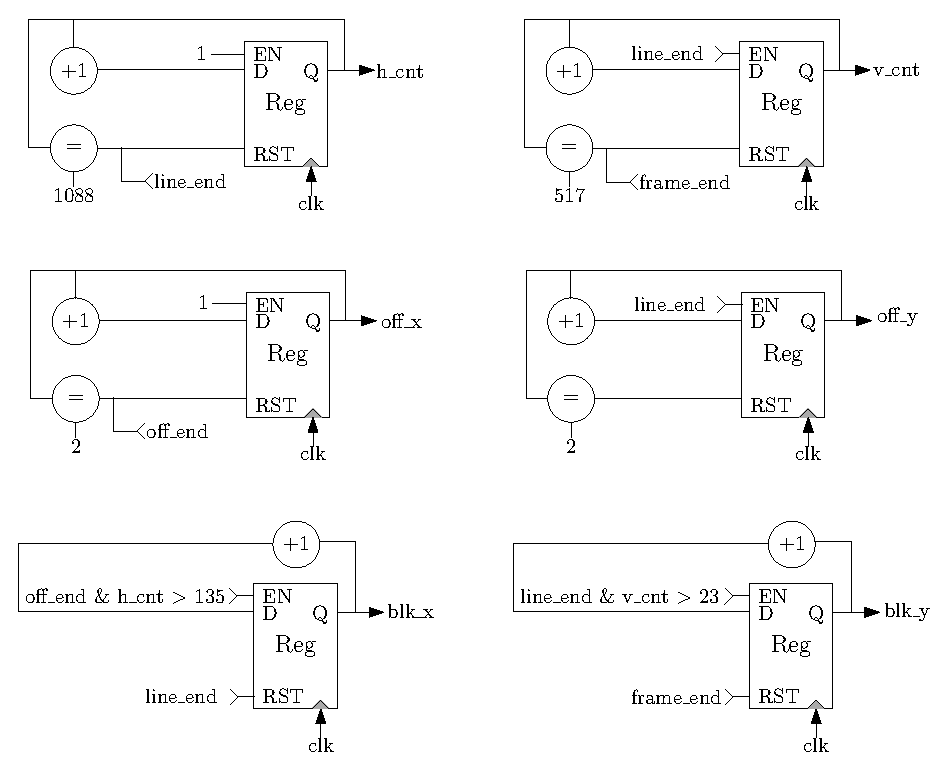
\includegraphics[width=\linewidth]{Chapter4-GPU_CLKU/res/gc_in}
    \caption{Graphic counter internal circuit}
    \label{fig:gpu/gc_in}
\end{figure}

\subsection{Synchronizer}

The synchronizer is in charge of generating the synchronization and display enable signals of the
VESA protocol. It simply looks at the values of the h\_cnt and v\_cnt signals provided by the 
graphic counter. If the values are within the ranges associated with the synchronizations or display
enable, the synchronizer sets the signal to high. As a reminder, the ranges were described in 
Figure \ref{fig:gpu/screen_vesa} and Table \ref{tab:gpu/vesa}. As the internal circuit is 
only a condition, it is not shown. The interface is shown in Figure \ref{fig:gpu/synchronizer}.  

\begin{figure}[H]
    \centering
    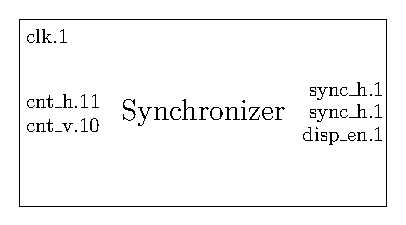
\includegraphics[scale=1.0]{Chapter4-GPU_CLKU/res/synchronizer}
    \caption{Synchronizer}
    \label{fig:gpu/synchronizer}
\end{figure}

\subsection{I2C HDMI Config}

This module is provided by Terasic to configure the HDMI controller present on the DE10 nano board. 
In this work, it is used as a library, i.e., its description is not detailed here since it has been used as a black box. In the GPU, it is simply connected to the pins of the physical
HDMI controller as Terasic suggests in its tutorial. The interface is provided in 
Figure \ref{fig:gpu/i2c}.

\begin{figure}[H]
    \centering
    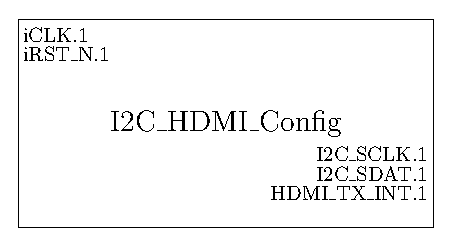
\includegraphics[scale=0.8]{Chapter4-GPU_CLKU/res/i2c}
    \caption{I2C HDMI Config}
    \label{fig:gpu/i2c}
\end{figure}

\subsection{Complete circuit}

The GPU whose internal circuit is given in Figure \ref{fig:gpu/gpu_in}, like the CPU, runs in 
sequence. It starts by reading the mask in the mask memory. Then it reads the tiles to be edited in 
the memory and shifts the masks at the same time. The results of these two operations arrive in the 
mask logic unit where they are processed in a combinatorial way. Each mask operates on the tile 
associated to it, taking into account the primary and secondary colors. Once this is done, the 
memory is enabled again, in writing mode this time. 

Similarly to some CPU memories, the mask memory has a MAU access that allows reading and writing of this 
memory from the ARM processor.

This constitutes the computational part of the GPU, the one that the CPU controls through its ST and 
LD operations. 

Then, there is the controller that fetches each tile in memory one by one and draws all the pixels
on the physical screen. 
It also manages the synchronization signals of the VESA protocol. The graphic counter is used to 
provide the address of the memory. To do this, the blk\_x and blk\_y outputs are concatenated to 
form the address. Then, the offsets are added together to form an index in the tile and select the current 
pixel. The selected pixel is then put on the output if the signal in\_memory of the graphic counter 
is high, otherwise the color is black. It is to this effect that the two multiplexers are used on 
the hdmi\_tx\_d output. It should be noted that the index and the im\_mem signal must be delayed so 
that they arrive at the multiplexers at the same time as the tile requested from the memory. This 
is why two registers are left on their way. The cnt\_h and cnt\_v signals go to the synchronizer 
which is responsible for generating the synchronization signals. And finally, there is also the 
I2C\_HDMI\_Config to configure the physical HDMI controller.

It should be noted that two clocks are present. On the computational side, it is the same clock as 
the CPU that is used to ensure that the two modules are synchronized. On the HDMI side, it is the 
VESA protocol clock that is used. It is called gpu\_clk. The GPU interface is available in Figure
\ref{fig:gpu/gpu}.

\begin{figure}[H]
    \centering
    
\includegraphics[width=\linewidth]{Chapter4-GPU_CLKU/res/gpu_in}
    \caption{GPU internal circuit}
    \label{fig:gpu/gpu_in}
\end{figure}

\begin{figure}[H]
    \centering
    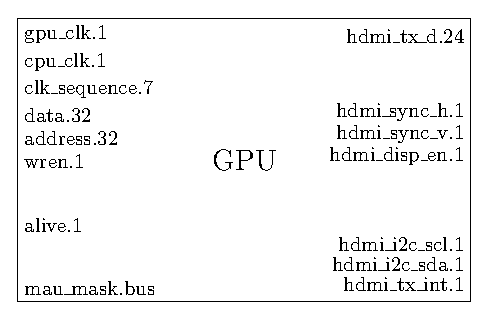
\includegraphics[scale=1.0]{Chapter4-GPU_CLKU/res/gpu}
    \caption{GPU}
    \label{fig:gpu/gpu}
\end{figure}

\section{Clock Unit (CLKU)}

As seen previously, two clocks are needed. One as high as possible for the CPU and the modules 
working synchronously with it and one for the 33.750MHz HDMI controller. The CPU clock cannot 
exceed 50MHz. Indeed, other higher frequencies have been tested but do not meet the timing 
constraints at compile time. For the CPU, the clock unit only passes the FPGA 50MHz physical clock 
from the input to the output (the CPU clock circuit is a simple wire). For the GPU clock, the frequency
has to be modified. This is done 
using a PLL (Phased-locked loop) which allows to generate a clock with a given frequency from 
another clock with a fixed frequency. This PLL is easily configured in a GUI using the Quartus 
Mega Wizard by setting the input and output frequencies. The CLKU then consists in a PLL. Its interface 
is given in Figure \ref{fig:clku/clku}.

\begin{figure}[H]
    \centering
    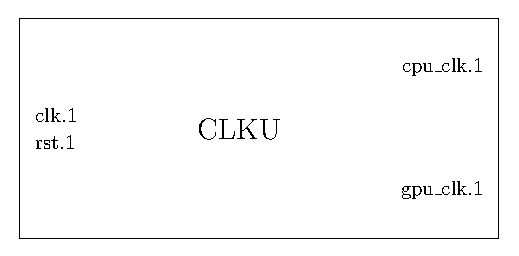
\includegraphics[scale=1.0]{Chapter4-GPU_CLKU/res/clku}
    \caption{CLKU}
    \label{fig:clku/clku}
\end{figure}
